\documentclass{beamer}
\usepackage[english]{babel}
\usepackage[utf8]{inputenc}
\mode<presentation>{\usetheme{FS18}}
\usepackage{amsmath,amsthm, amssymb, latexsym}
\usepackage[orientation=portrait,size=a0,scale=1.4]{beamerposter}
\usepackage{natbib}
\bibliographystyle{unsrt}
\usepackage{subcaption}
\graphicspath{{../figures/graphics/}}
 
\title{Local Variance Optimization for the Autonomous Regulation of Echo State Networks}
\author{Fabian Schubert, Claudius Gros}
\institute{Institute for Theoretical Physics, Goethe University Frankfurt a.M.}
\date{}

\renewcommand{\vec}[1]{\mathbf{#1}}

\newcommand{\vx}{\vec{x}}
\newcommand{\vy}{\vec{y}}
\newcommand{\vf}{\vec{f}}
\newcommand{\vsigm}{\boldsymbol{\sigma}}

\newcommand{\Err}{\mathrm{Err}}
\newcommand{\Exp}{\mathrm{E}}
\newcommand{\Var}{\mathrm{Var}}

\newcommand{\avgt}[1]{\left< #1 \right>_T}
\newcommand{\avgp}[1]{\left< #1 \right>_P}


\begin{document}
\begin{frame}[t]
\begin{columns}[t]
\begin{column}{.4\textwidth}
\begin{myblock}{Introduction}
\begin{itemize}
	\item Echo state networks have proven to be a powerful tool in the field of time series prediction~\citep{Jaeger_2001}.
	\item The spectral radius $|\Lambda_{\rm max}|$ of the synaptic weight matrix provides a measure to regulate the network in an appropriate working regime~\cite{Caluwaerts_2013}. We show that $|\Lambda_{\rm max}|$ can be regulated by local homeostasis of the variance $\sigma_y^2$ of neural activity. This variance control operates on the gain of the neural transfer function and its optimization target depends on the variance $\sigma_{\rm ext}^2$ of external input.
	\item In contrast to previously proposed optimization rules via local intrinsic plasticity, our model relies on the assumption that external and recurrent input signals can be treated as two separate streams of information. The network can hence react autonomously to changes of the input statistics.
\end{itemize}
\end{myblock}

\begin{myblock}{Model Description}
\vspace{-30pt}
\begin{align*}
y_i^{t+1} &= \mathrm{tanh}\left( a_i^t X_i^{t+1} \right) &
X_i^{t+1} &= \sum_{j=1}^{N} W_{ij} y_j^t + E_i^{t+1}  \\
b_i^{t+1} &= b_i^t + \epsilon_{b} \left[ \avgt{y_i} - \mu_{t} \right] &
a_i^{t+1} &= a_i^{t} + \epsilon_{a} \left[ \sigma_{t}^2 - \left( y_i^t - \overline{y}(t)_i\right)^2 \right]  \\
\overline{y}^{t+1}_i &= \epsilon_{\rm trail} \left[ y_i^{t+1} - \overline{y}^{t}_i\right]
\end{align*}
\begin{figure}
	\centering
	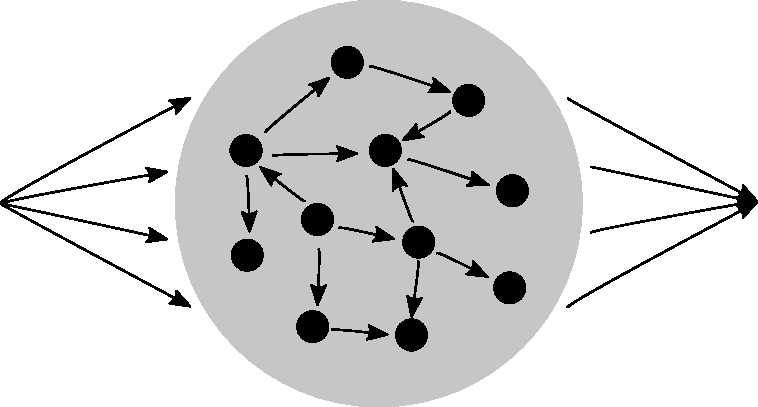
\includegraphics[width=0.5\textwidth]{../figures/illustration.pdf}
\end{figure}
\begin{itemize}
	\item $W_{ij}$ is a sparse random matrix with connection probability $p$. Nonzero entries were drawn from a Gaussian distribution $\mathcal{N}(\mu = 0,\sigma = 1/\sqrt{N p})$. Diagonal entries were always set to zero.
	\item $E^t_{i}$ are random vectors of size $N$ with independent entries drawn from a Gaussian distribution $\mathcal{N}(\mu = 0,\sigma = \sigma_{\rm ext})$.
	\item By changing individual gain and bias values $a_i$ and $b_i$, the homeostatic control tries to drive the activity standard deviation and mean of every cell to the value given by $\sigma_{t}$ and $\mu_{t}$.
	\item By controlling the output variance of the neural activity, we can tune the network into a regime that exhibits subcritical, but transiently active dynamics in the absence of external input.
	\item This led to the question how a homeostatic variance control could be used to tune network properties into a desired regime, even under changing input statistics. 
\end{itemize}
\end{myblock}

\begin{myblock}{Self-Consistency Equation}
	If we assume no correlations in time across the neural population, we can formulate a self-consistency equation, given by
	\begin{equation*}
	\sigma^2_{t} = \int_{-\infty}^{\infty}  \tanh^2\left(ay\right) \mathcal{N}\left(y, \mu = 0, \sigma = \sqrt{\sigma^2_{t} + \sigma^2_{\rm ext}}\right)	\mathrm{d}y \;. 
	\end{equation*}
	
	A useful approximation with the correct scaling to second order as well as the right convergence is $\tanh^2(x) \approx 1 - \exp\left(-x^2 \right)$.
	
	From this approximation we can derive a relation between a target variance $\sigma_{t}$ and the external input variance $\sigma_{\rm ext}$ that marks the point where the spectral radius is unity:
	
	\begin{equation*}
	\sigma_{\rm t} \approx \left[\sqrt{\frac{3}{2}} \frac{\sigma_{\rm w}}{\sigma_{\rm ext}} +1\right]^{-1/2} \; .
	\end{equation*}
	This approximate solution is shown in Fig.~\ref{fig:sweep_sim}.
\end{myblock}

\begin{myblock}{Scaling of Spectral Radius for Inhomogeneous Gains}
	\vspace{-30pt}
	\begin{figure}
		\centering
		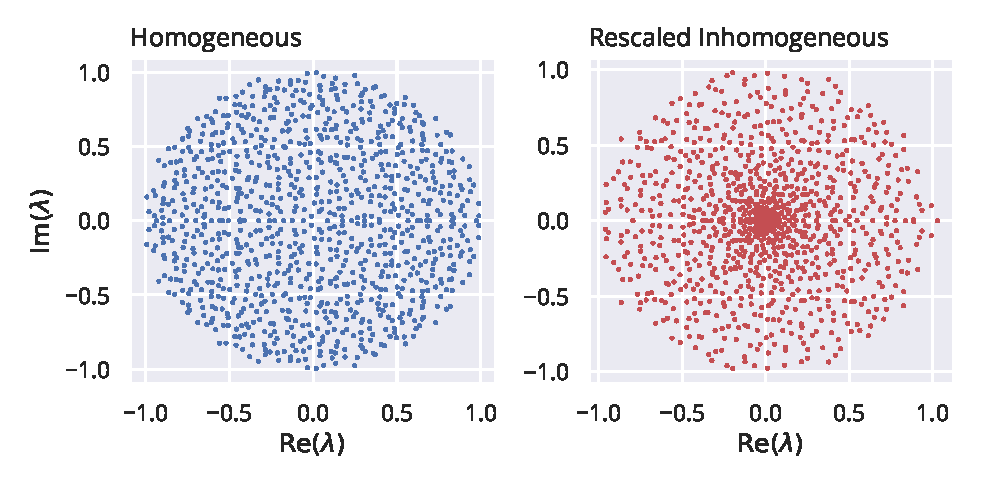
\includegraphics[width=\textwidth]{../figures/eigvals.pdf}
		\caption{A: Distribution of eigenvalues for all gains set to $1$. B: Gains drawn from a uniform distribution, such that $\sqrt{\sum_i a^2_i/N} = 1$.}		
	\end{figure}
	In the self-consistency equation, we assumed a single gain parameter $a$ controlling the spectral radius. For an \emph{inhomogeneous} distribution of gains, we found that the spectral radius is preserved if $\sqrt{\sum_i a^2_i/N}$ remains constant. However, inhomogeneity caused a bunching of eigenvalues towards zero and reduced the task performance of the network.
\end{myblock}

\end{column}



\begin{column}{.55\textwidth}
%\begin{myblock}{Network Dynamics}
%	\begin{figure}
%		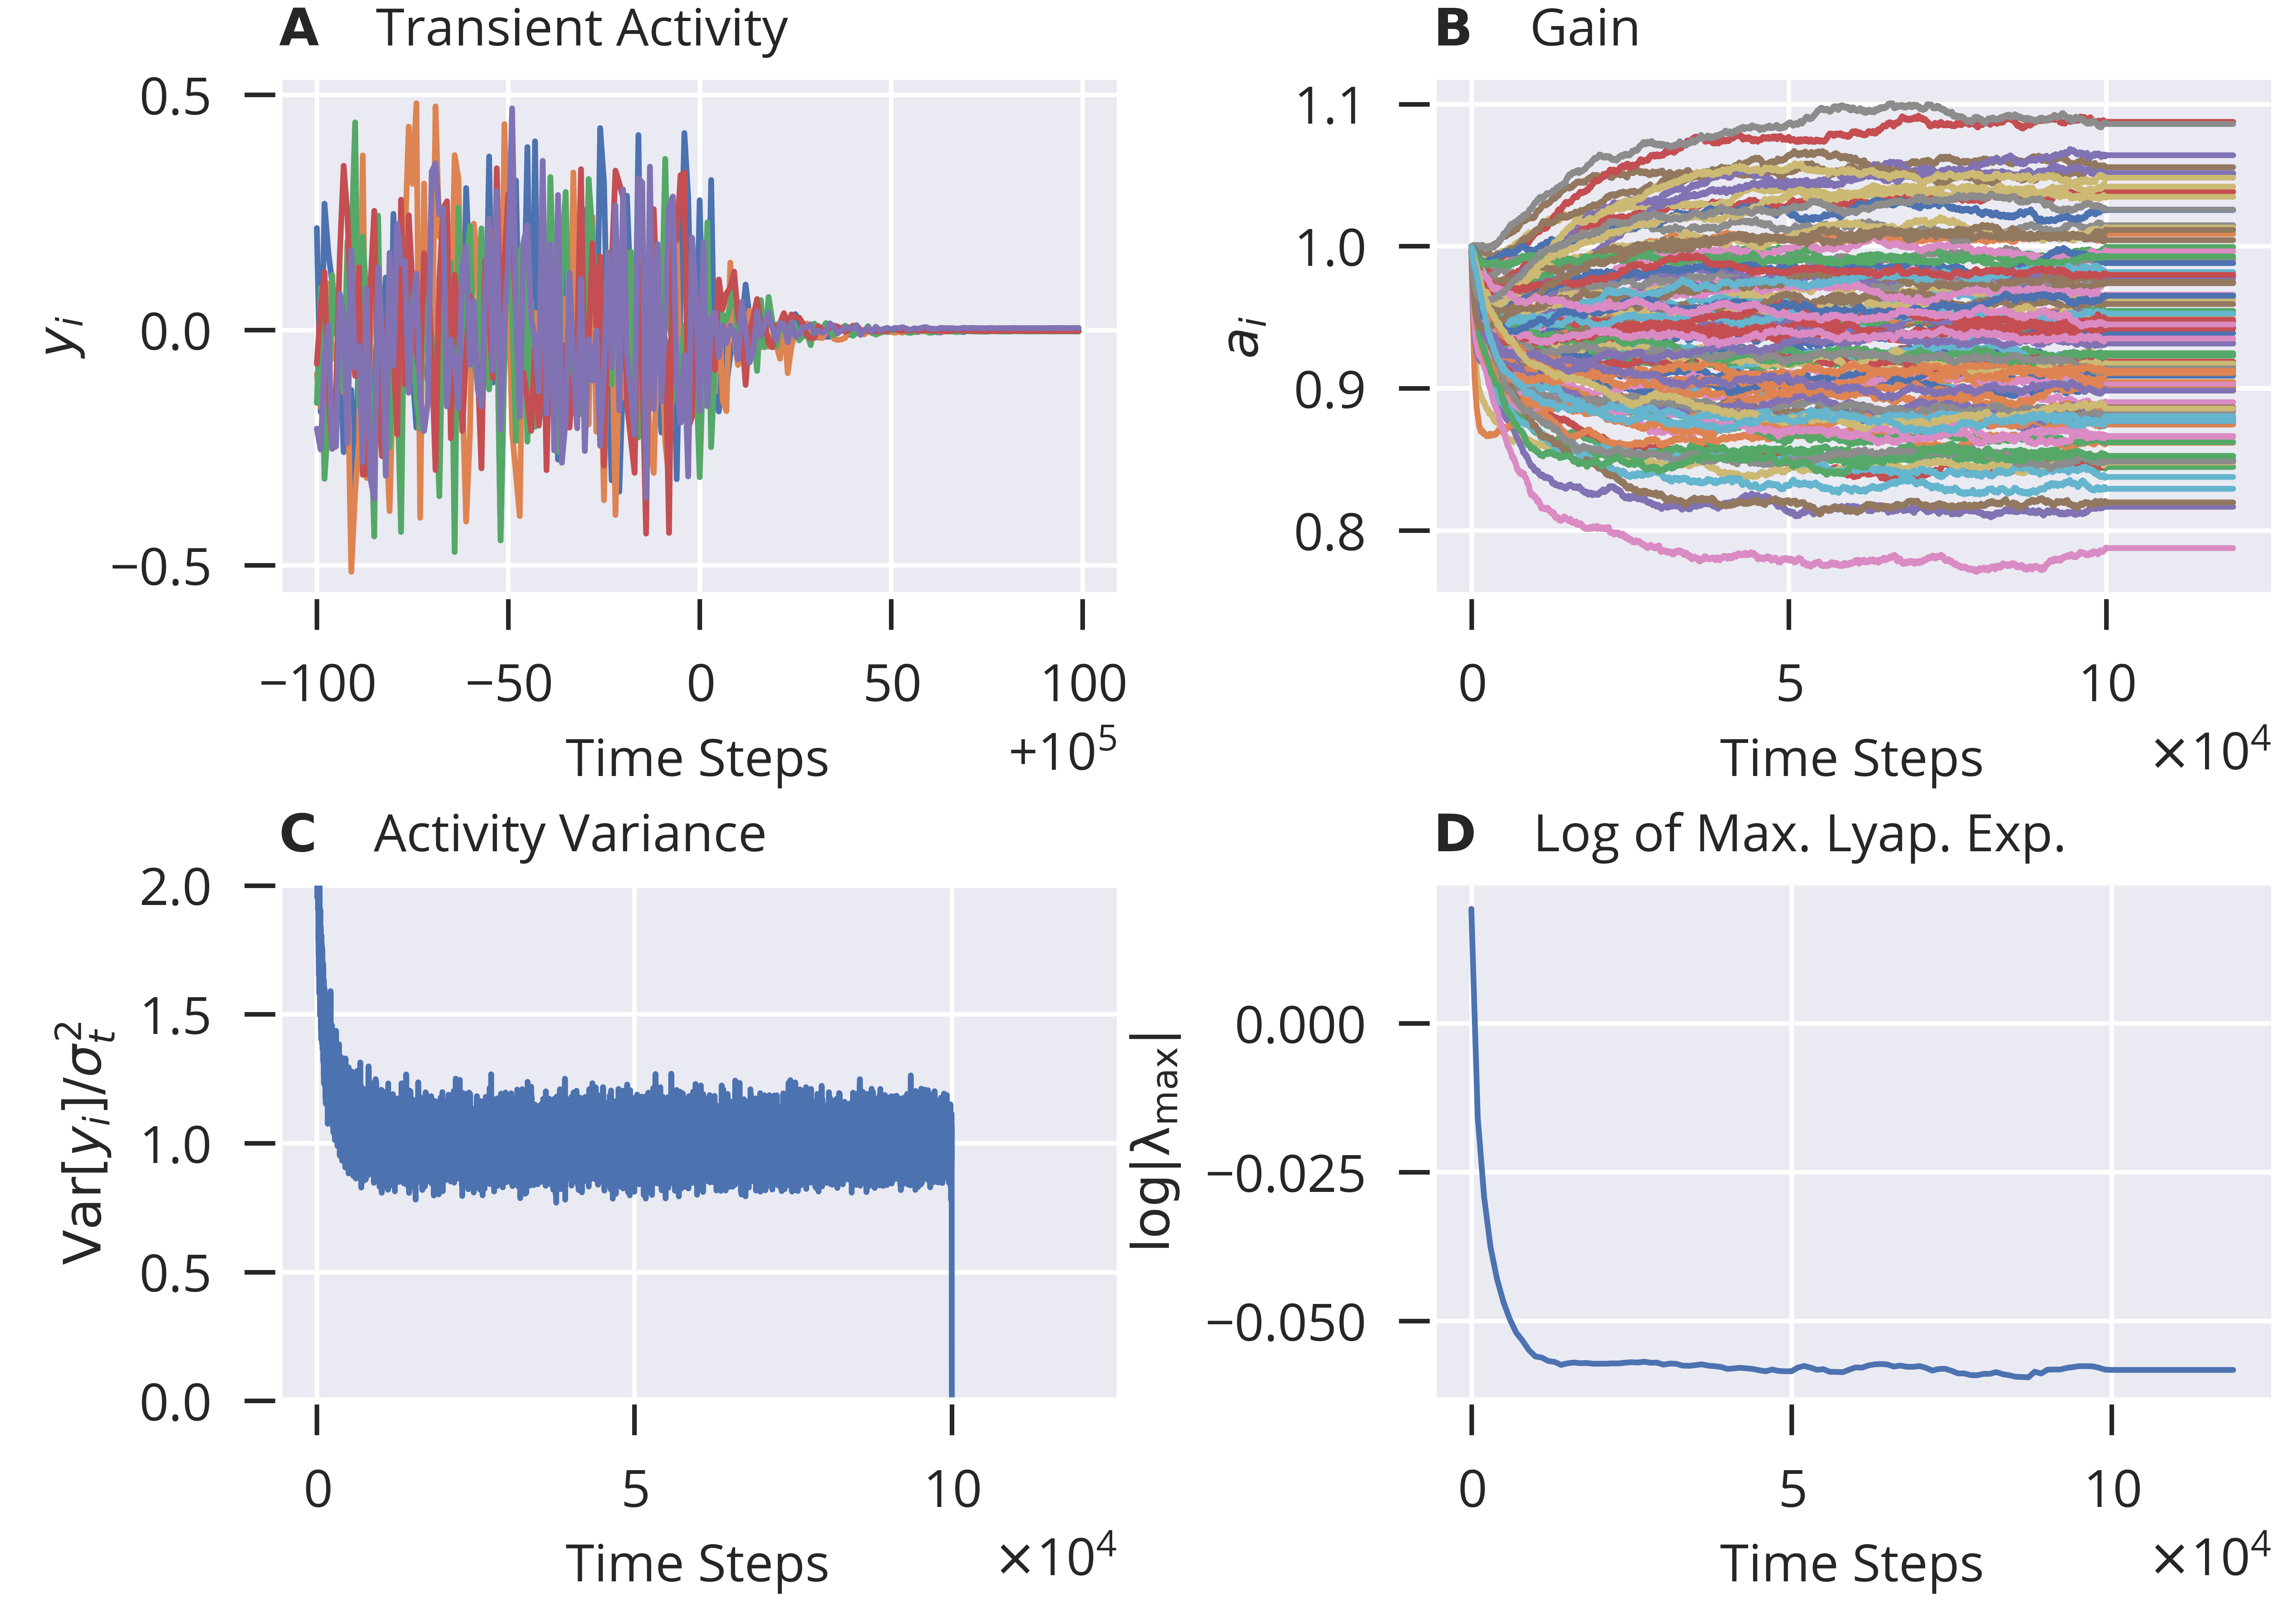
\includegraphics[width=0.9\textwidth]{../figures/res_comp.png}
%		\caption{Exemplary network dynamics, where the external input was switched off after $10^5$ time steps, followed by a transient period of decaying activity.}
%		\label{fig:trans_dyn}
%	\end{figure}
%\end{myblock}	

%\begin{myblock}{Nontrivial Memory Task}
%	\begin{itemize}
%		\item We defined a XOR-Memory recall task given by $f(t) = \mathrm{XOR}\left[u(t-\tau),u(t-\tau-1)\right]$.
%		\item We tested the performance of the ESN after homeostasis has equilibrated for different pairs of input and target variances, see Fig.~\ref{fig:sweep_sim}.
%		\item The analytically derived expression provides a good fit to the optimal performance marked by the orange line.
%	\end{itemize}
%\end{myblock}
\vspace{-8pt}
\begin{myblock}{Nontrivial Memory Task}
	
	\begin{figure}
		\begin{minipage}[c]{0.5\textwidth}
			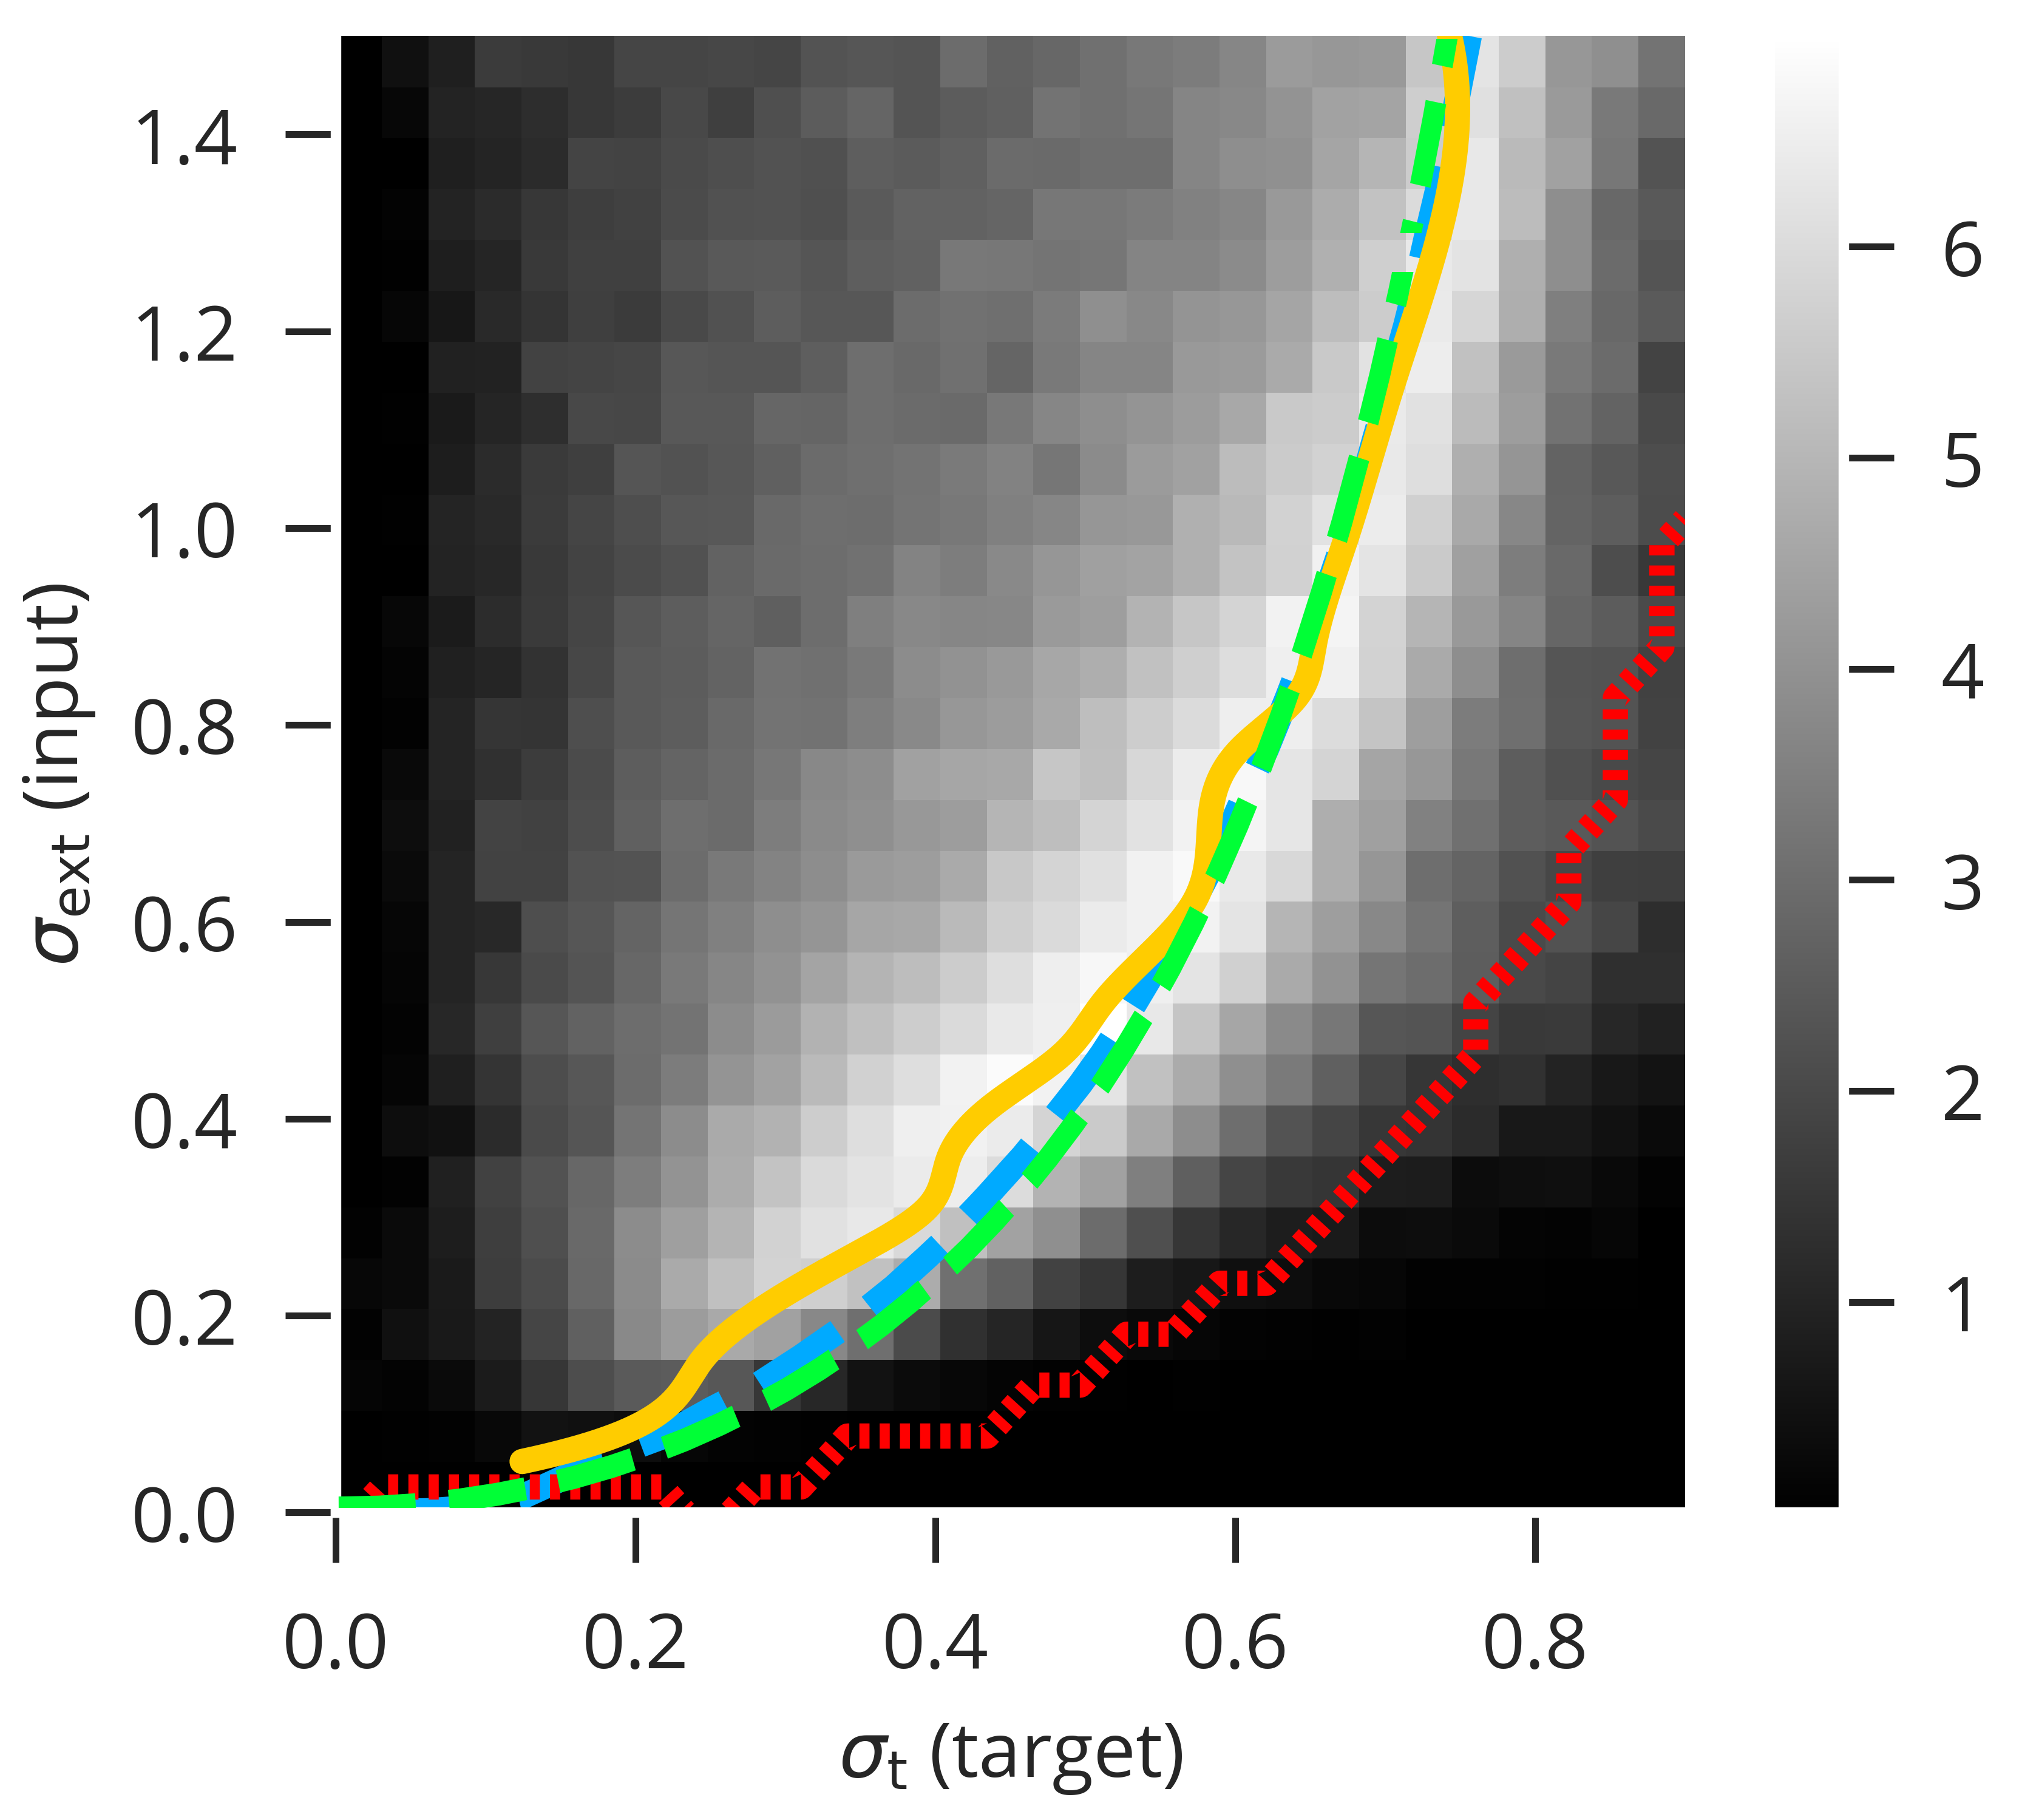
\includegraphics[width=\textwidth]{../figures/xor_task.png}
		\end{minipage}\hfill
		\begin{minipage}[l]{0.5\textwidth}
			\begin{itemize}
				\item We defined a XOR-Memory recall task given by $f(t) = \mathrm{XOR}\left[u(t-\tau),u(t-\tau-1)\right]$.
				\item We tested the performance of the ESN after homeostasis has equilibrated for different pairs of input and target variances, see Fig.~\ref{fig:sweep_sim}.
				\item The analytically derived expression provides a good fit to the optimal performance marked by the orange line.
			\end{itemize}
			\vspace{10pt}
			\caption{XOR - Memory capacity, orange line marks max. MC for a given $\sigma_{\rm ext}$, red line the loss of the echo state property. The blue line marks where the spectral radius is unity, the green line is our analytically derived prediction. The loss of the echo state property is marked by the red line.}
			\label{fig:sweep_sim}
		\end{minipage}
	\end{figure}
	
	%\begin{figure}
	%	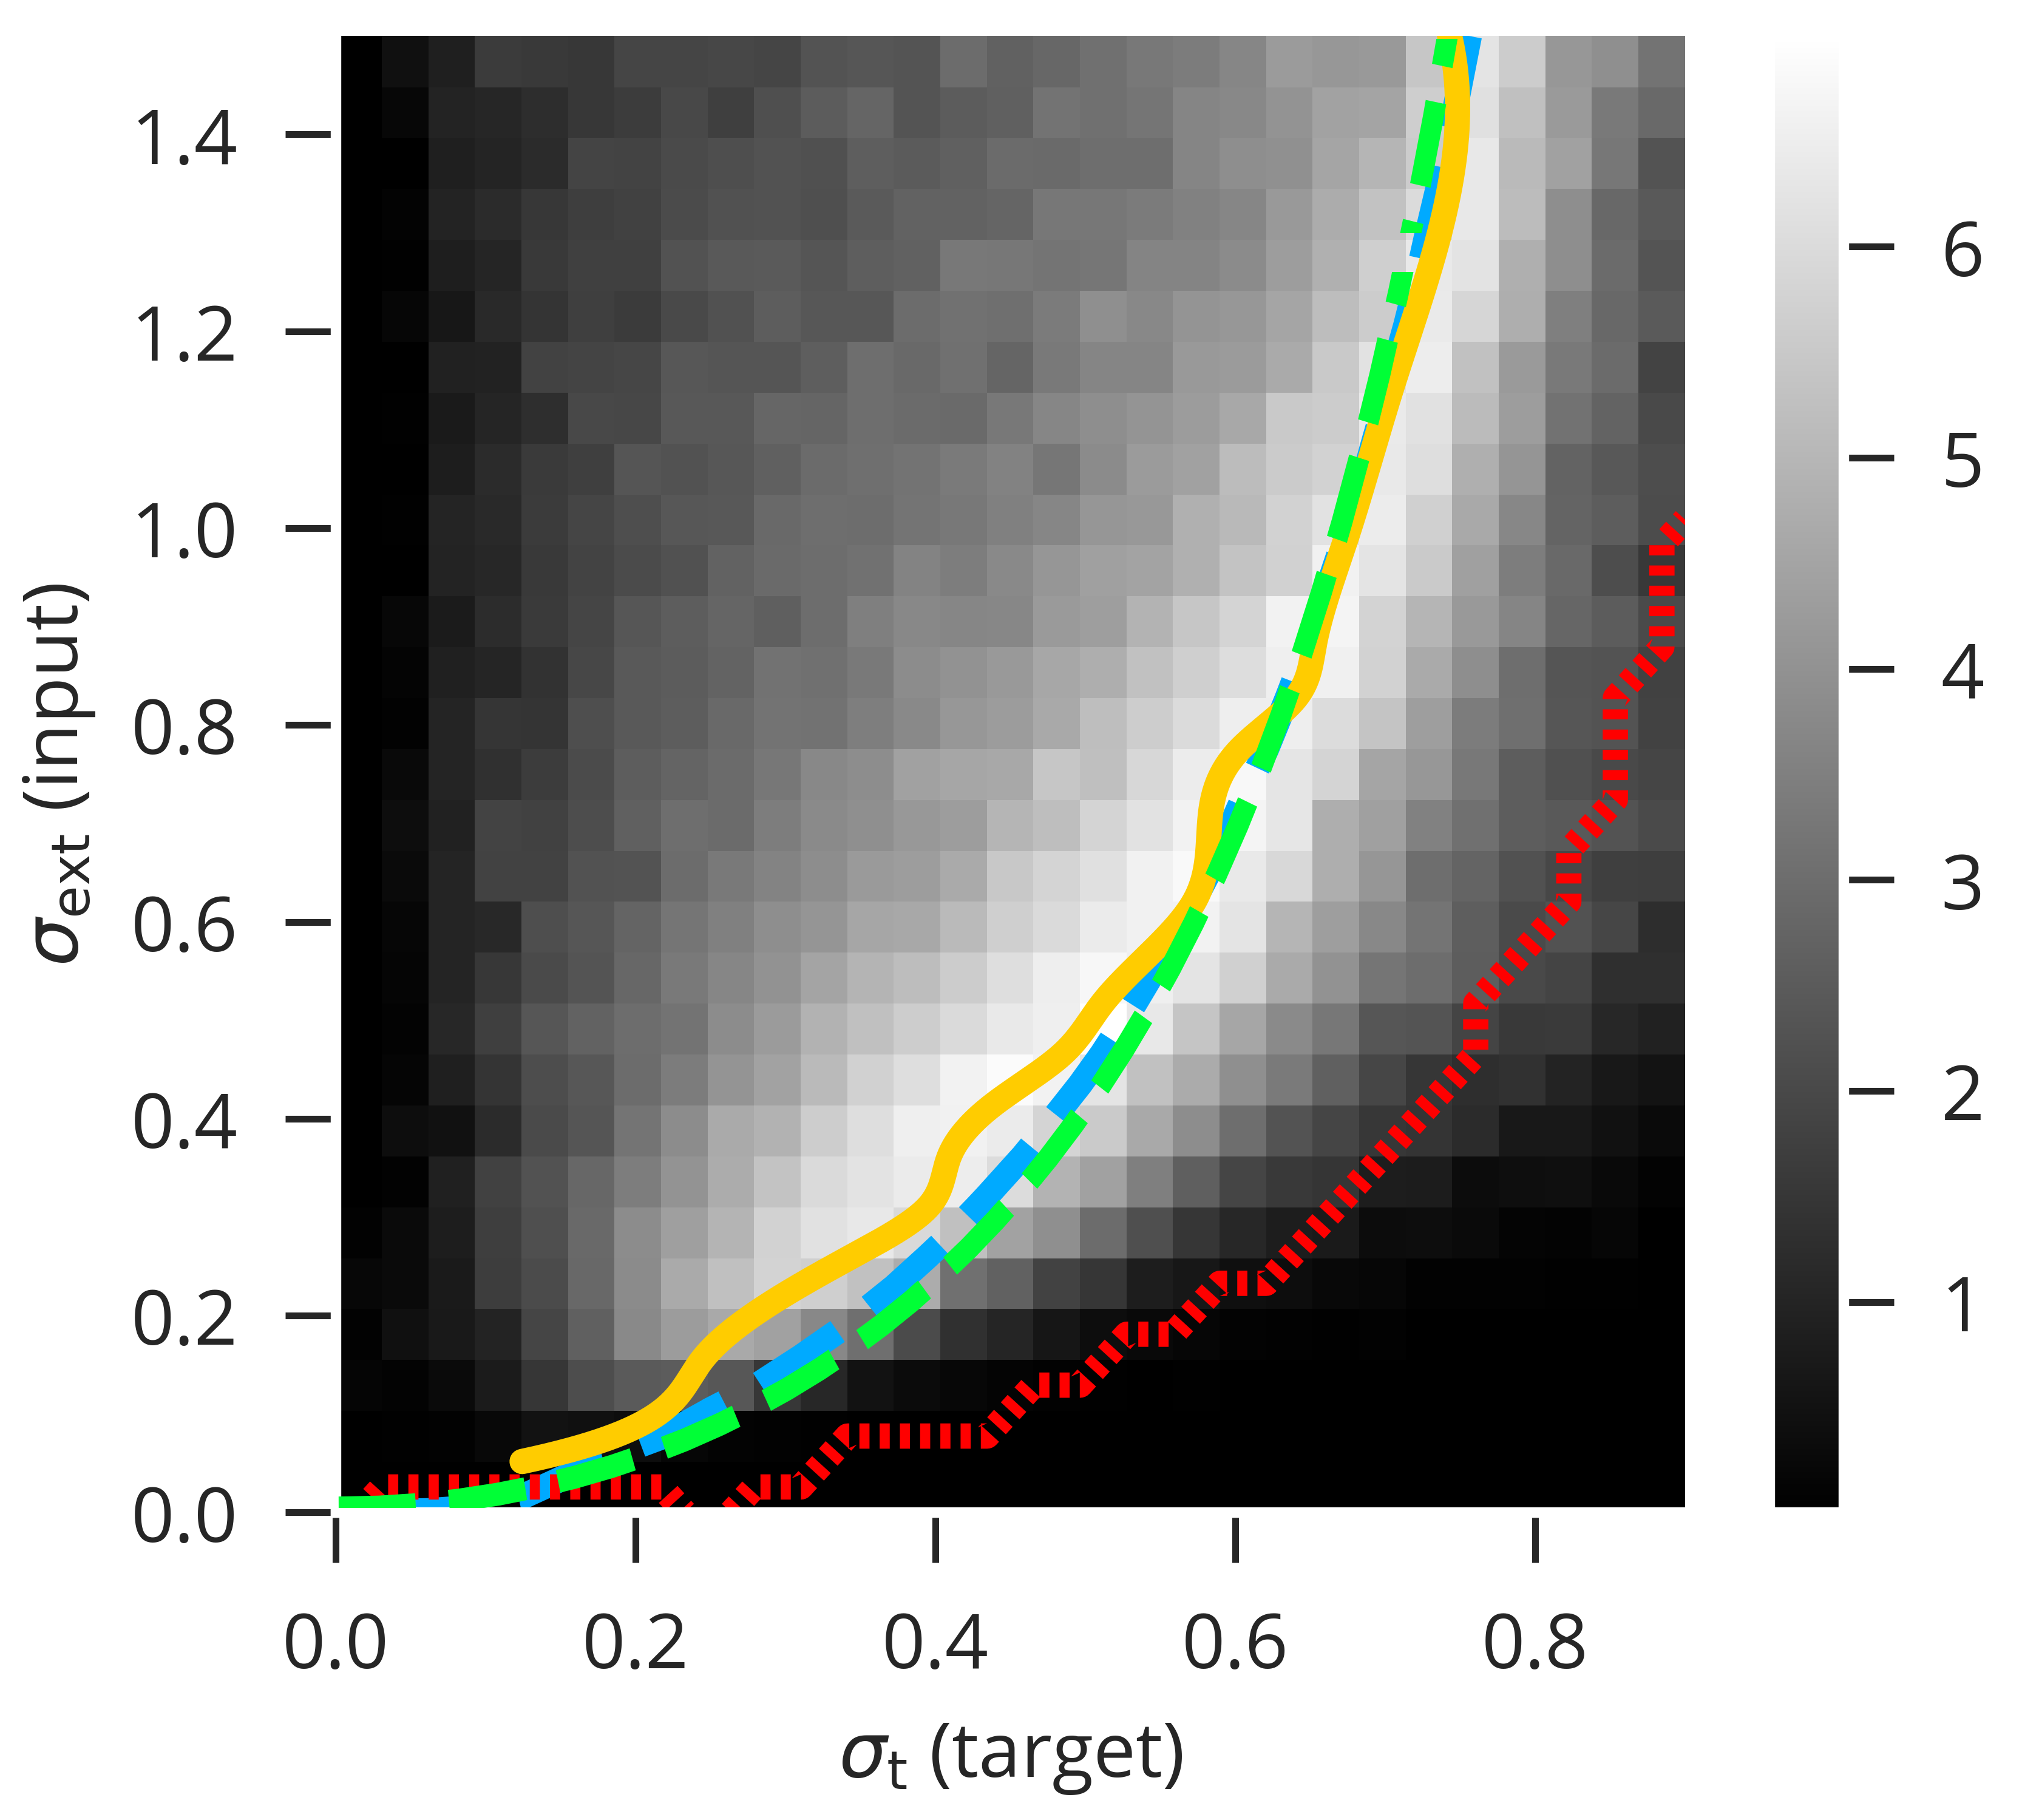
\includegraphics[width=0.48\textwidth]{../figures/xor_task.png}
	%	\caption{XOR - Memory capacity, orange line marks max. MC for a given $\sigma_{\rm ext}$, red line the loss of the echo state property. The blue line marks where the spectral radius is unity, the green line is our analytically derived prediction. The loss of the echo state property is marked by the red line.}
	%	\label{fig:sweep_sim}
	%\end{figure}
\end{myblock}

\begin{myblock}{Gain Optimization: Local vs Full Gradient}
	
	\begin{itemize}
		\item We were interested in the gain adaptation dynamics for our particular task. In particular, we compared a simplified, local a error gradient based gain adaptation against its full counterpart.
		\item We calculated the full gradient using the Realtime-Recurrent-Learning (RTRL) scheme with a squared error loss function $\mathcal{L}$. The nonlocal term was dropped in the approximate rule.
		\vspace{5pt}
		\begin{align*}
		\mathcal{L} &= \left\langle \frac{1}{2} \epsilon^2(t)\right\rangle_t = \left\langle \frac{1}{2} \left( \mathbf{w}_{\rm out} \mathbf{y}(t) - f(t)\right)^2\right\rangle_t \\
		\Delta a &= \partial_a \mathcal{L} = \left\langle \epsilon(t) \mathbf{w}_{\rm out} \partial_a \mathbf{y}(t) \right\rangle_t \\
		\partial_a \mathbf{y}(t) &= \mathbf{y}'(t) \ast \left[ \mathbf{X}(t) + a \mathrm{W} \partial_a \mathbf{y}(t-1)\right] \\
		\Delta a_{\rm approx} &= \left\langle \epsilon(t) \mathbf{w}_{\rm out} \mathbf{y}'(t) \ast \mathbf{X}(t) \right\rangle_t \\
		y'_i(t) &= 1-y^2(t)
		\end{align*}
		\item This approximation is similar to recently proposed local synaptic learning rules for recurrent networks \cite{Murray_2019}.
	\end{itemize}
	
	\begin{figure}
		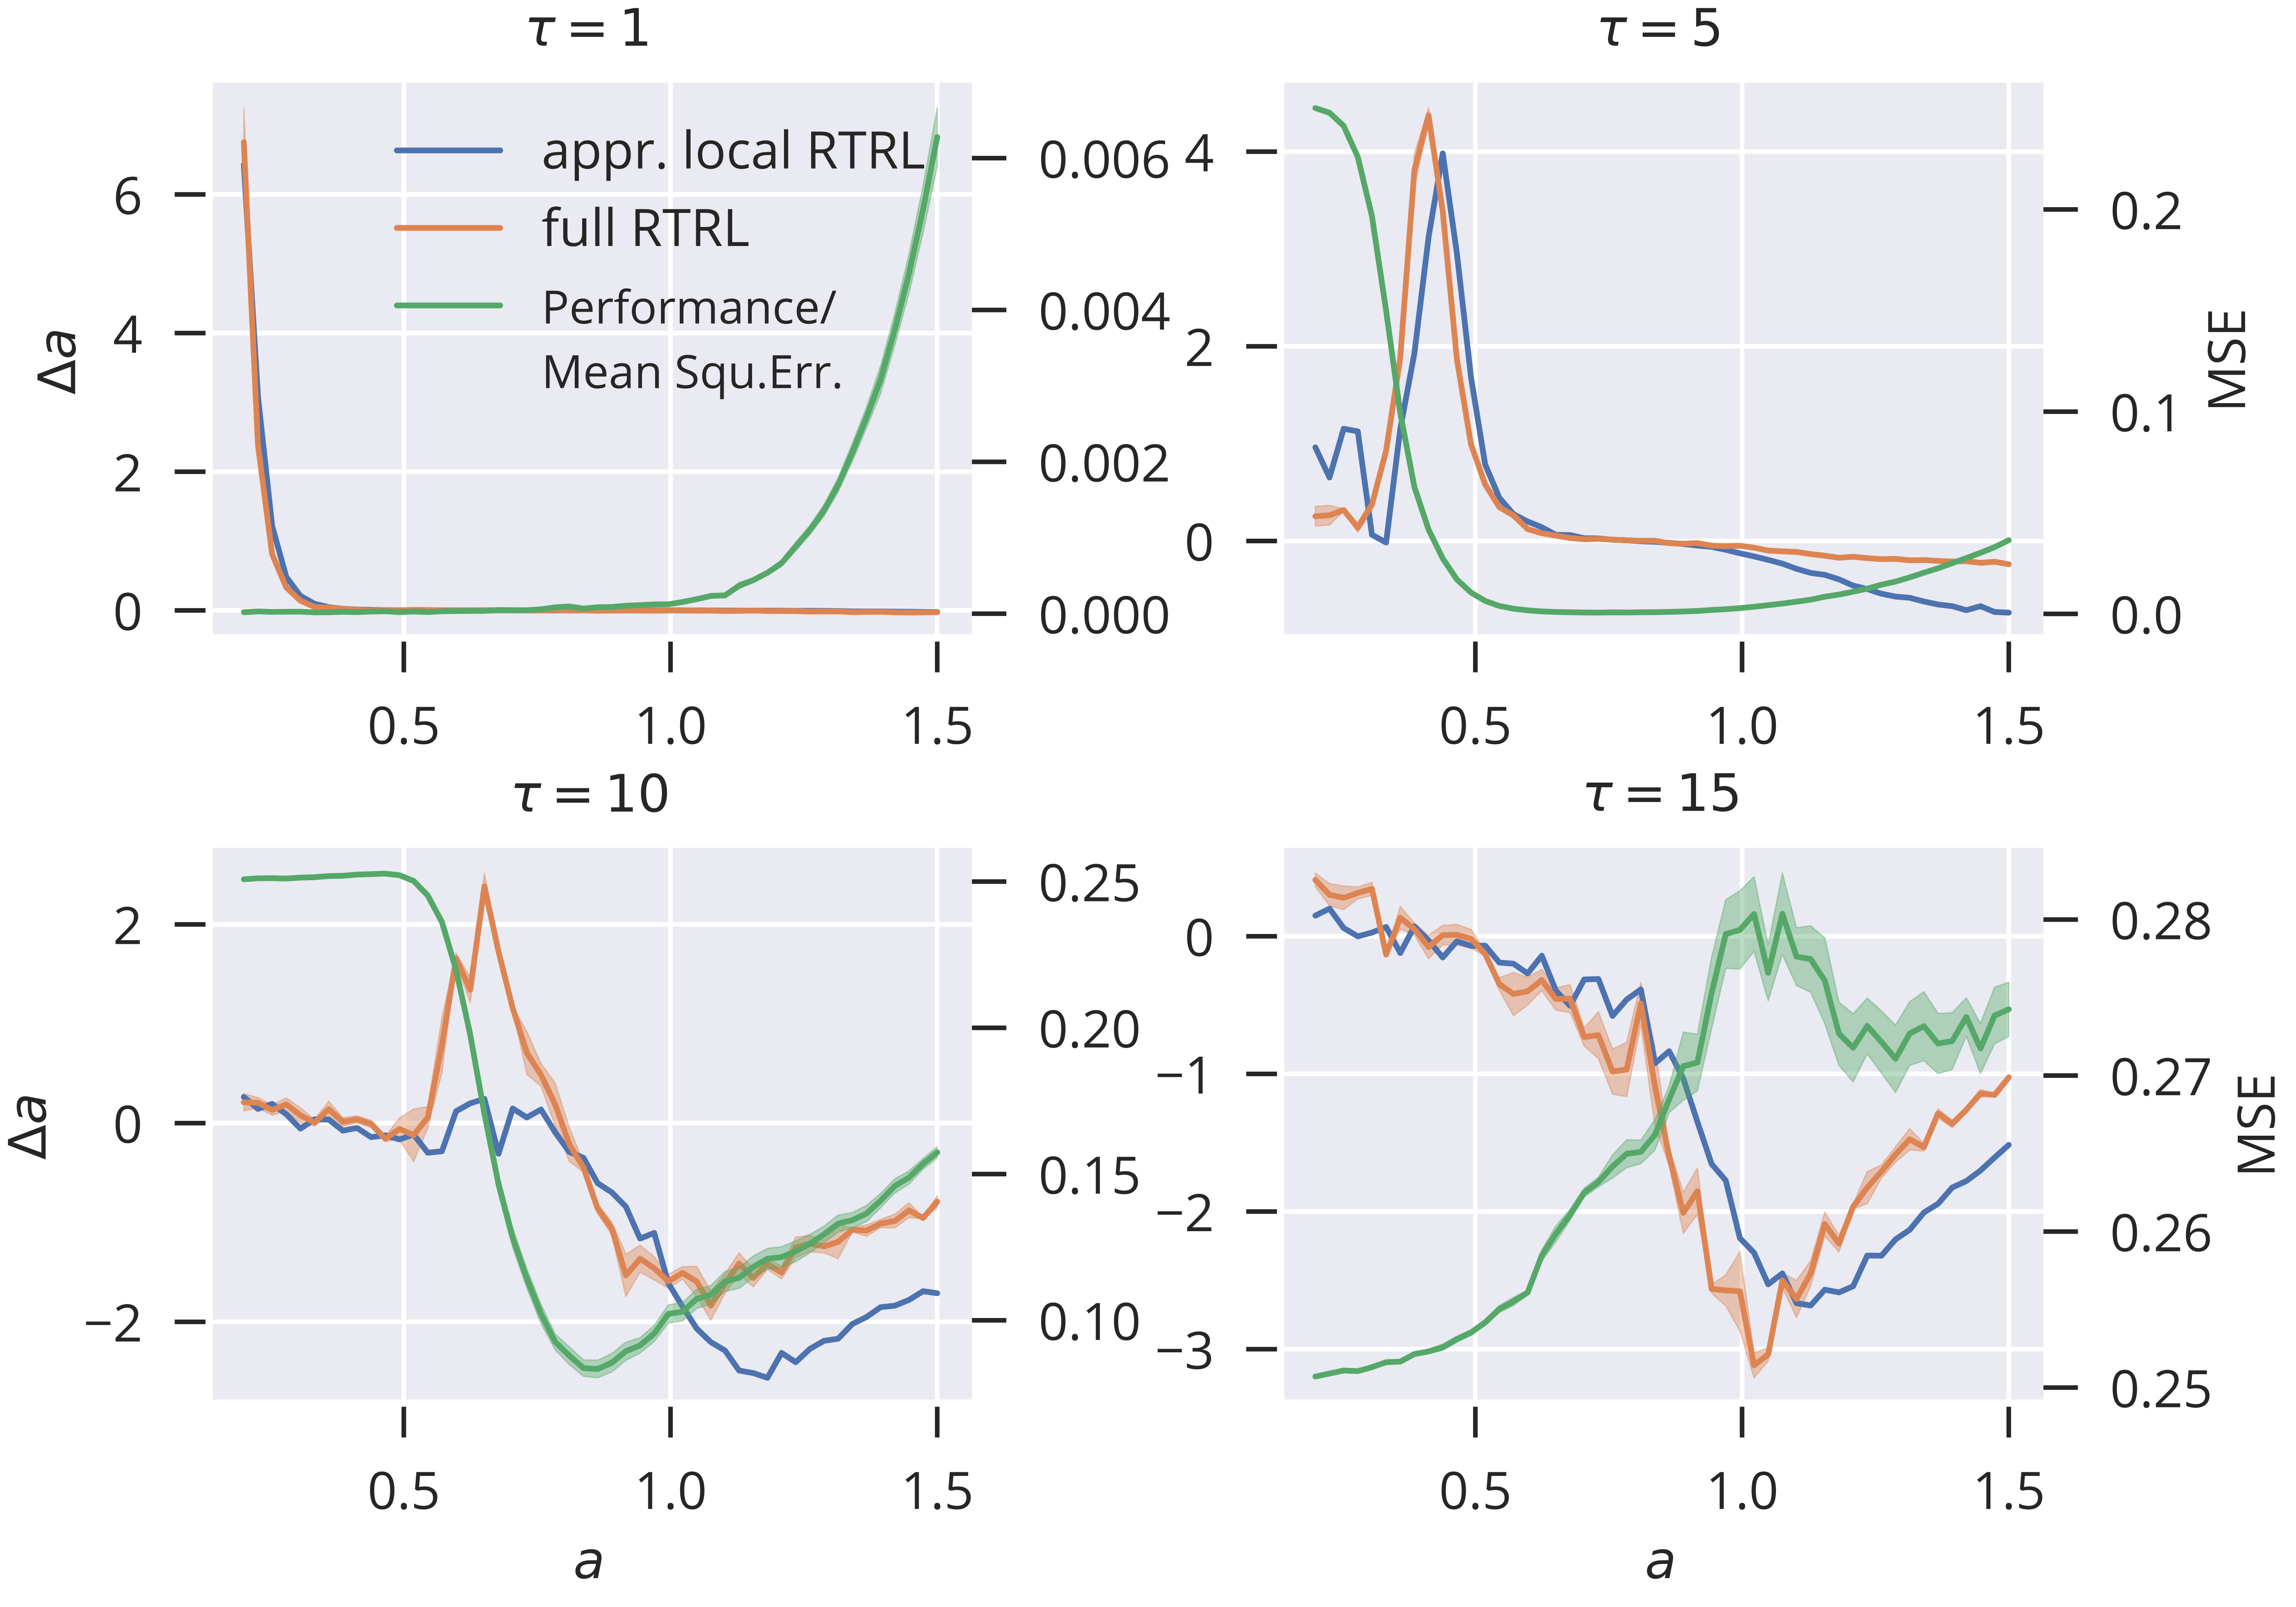
\includegraphics[width=0.9\textwidth]{../figures/delta_a_local_fix.png}
		\caption{Gradient based update rules for the gain parameter $a$: Full gradient (orange) vs.local approximation (blue).}
		\label{fig:delta_a_sim}
	\end{figure}
\end{myblock}

\begin{myblock}{Outlook: Homeostasis and Error-Driven Gain Optimization}
	\begin{itemize}
	\item Combining our homeostatic update rule with the error-driven approach might help to avoid the ``trivial" fixpoint of zero gains.
	\item Furthermore, tuning the network into a state close to the critical transition provides a good starting point for error-driven optimization. 
	\end{itemize}
\end{myblock}


\begin{myblock}{References}
	\scriptsize
	\bibliography{../../../../../lit_base.bib}
\end{myblock}

\end{column}
\end{columns}
\end{frame}
\end{document}
